\section{Dataset and Preprocessing}
\label{sec:dataset}

\subsection{The BDLitchi Benchmark Corpus}
All empirical evaluations in this investigation are established upon the publicly released BDLitchi corpus \cite{litchi_dataset_2022}, captured across commercial litchi orchards located in Dinajpur ($25.6279^\circ\,\text{N}, 88.6332^\circ\,\text{E}$) and Ishwardi ($24.1292^\circ\,\text{N}, 89.0683^\circ\,\text{E}$), Bangladesh. The dataset comprises \totalImages{} high-resolution RGB photographs collected under diverse natural field conditions, encompassing varying solar angles, natural canopy shade, complex soil-weed backgrounds, and diverse stages of plant phenology.

\begin{figure}[t]
\centering
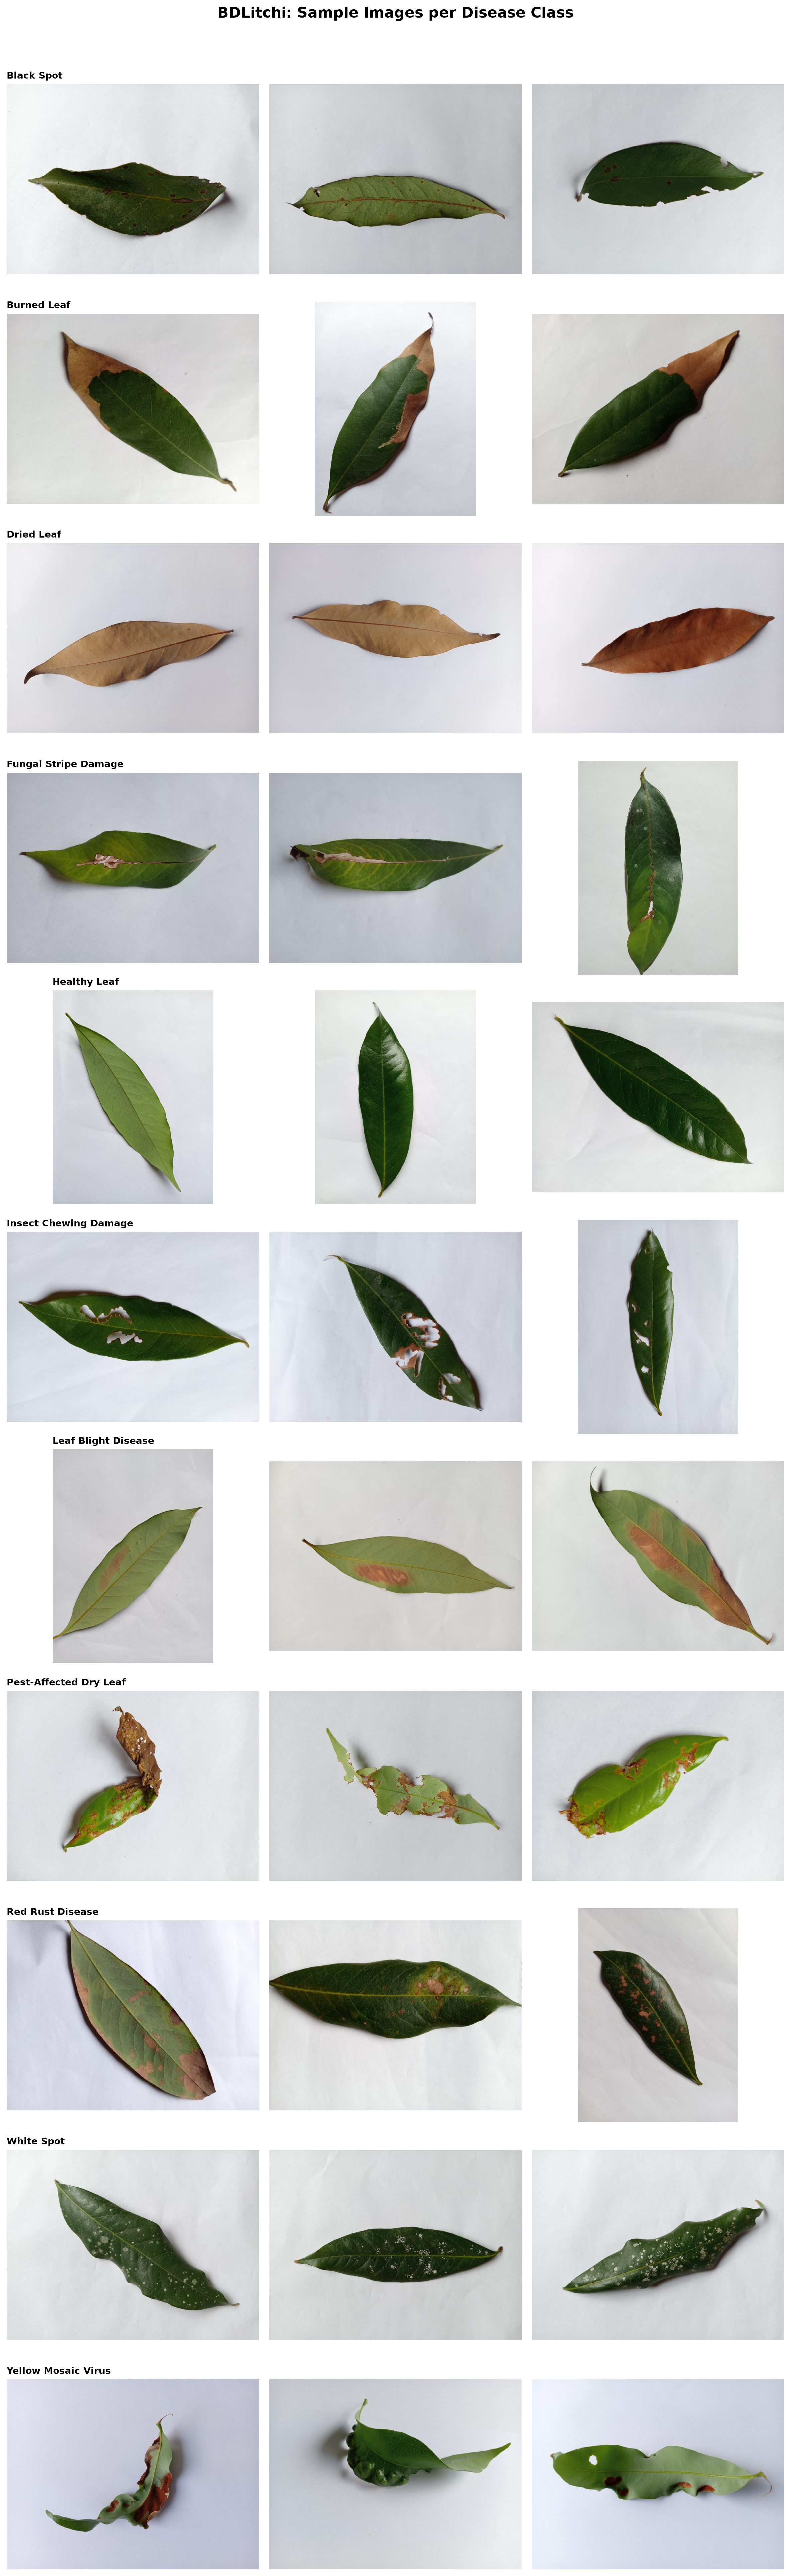
\includegraphics[width=\columnwidth]{figures/sample_grid.png}
\caption{Representative natural field images from the BDLitchi dataset illustrating the \numClasses{} foliar health and disease categories under uncontrolled orchard lighting, variable leaf orientations, and complex canopy clutter.}
\label{fig:sample_grid}
\end{figure}

The corpus encompasses \numClasses{} distinct diagnostic categories, comprising 10 foliar pathologies and 1 healthy reference category:
\begin{enumerate}
    \item \textbf{Black Spot:} Circular to irregular dark brown-to-black necrotic lesions on the adaxial surface caused by foliar fungal colonization.
    \item \textbf{Burned Leaf:} Extensive marginal and apical leaf scorching triggered by intense solar radiation and extreme atmospheric moisture deficits.
    \item \textbf{Dried Leaf:} Complete loss of cellular turgor, desiccation, and curling of mature leaves resulting from severe vascular compromise.
    \item \textbf{Fungal Stripe Damage:} Elongated chlorotic-to-necrotic parallel stripes tracking the primary longitudinal leaf veins.
    \item \textbf{Healthy Leaf Lamina:} Vigorous, unblemished leaf lamina with uniform chlorophyll distribution and intact epidermal morphology.
    \item \textbf{Insect Chewing Damage:} Irregular macroscopic holes, jagged margins, and windowpane skeletonization caused by herbivorous caterpillar and beetle feeding.
    \item \textbf{Leaf Blight Disease:} Rapidly expanding water-soaked necrotic patches with dark brown concentric rings, primarily attributed to \textit{Phomopsis} or \textit{Alternaria} complex.
    \item \textbf{Pest-Affected Dry Leaf:} Combined pathological symptoms presenting localized insect galling and necrotic punctures accompanied by regional leaf desiccation.
    \item \textbf{Red Rust Disease:} Powdery, velvet-like orange-red algal pustules erupted across the lamina, characteristic of parasitic \textit{Cephaleuros virescens}.
    \item \textbf{White Spot:} Punctate, chalky white-to-pale-gray circular spots with dark brown halos, representing early-stage fungal spot development.
    \item \textbf{Yellow Mosaic Virus:} Systemic vein clearing, vivid yellow-green mottled variegation, and leaf crinkling resulting from viral infection.
\end{enumerate}

\begin{figure}[t]
\centering
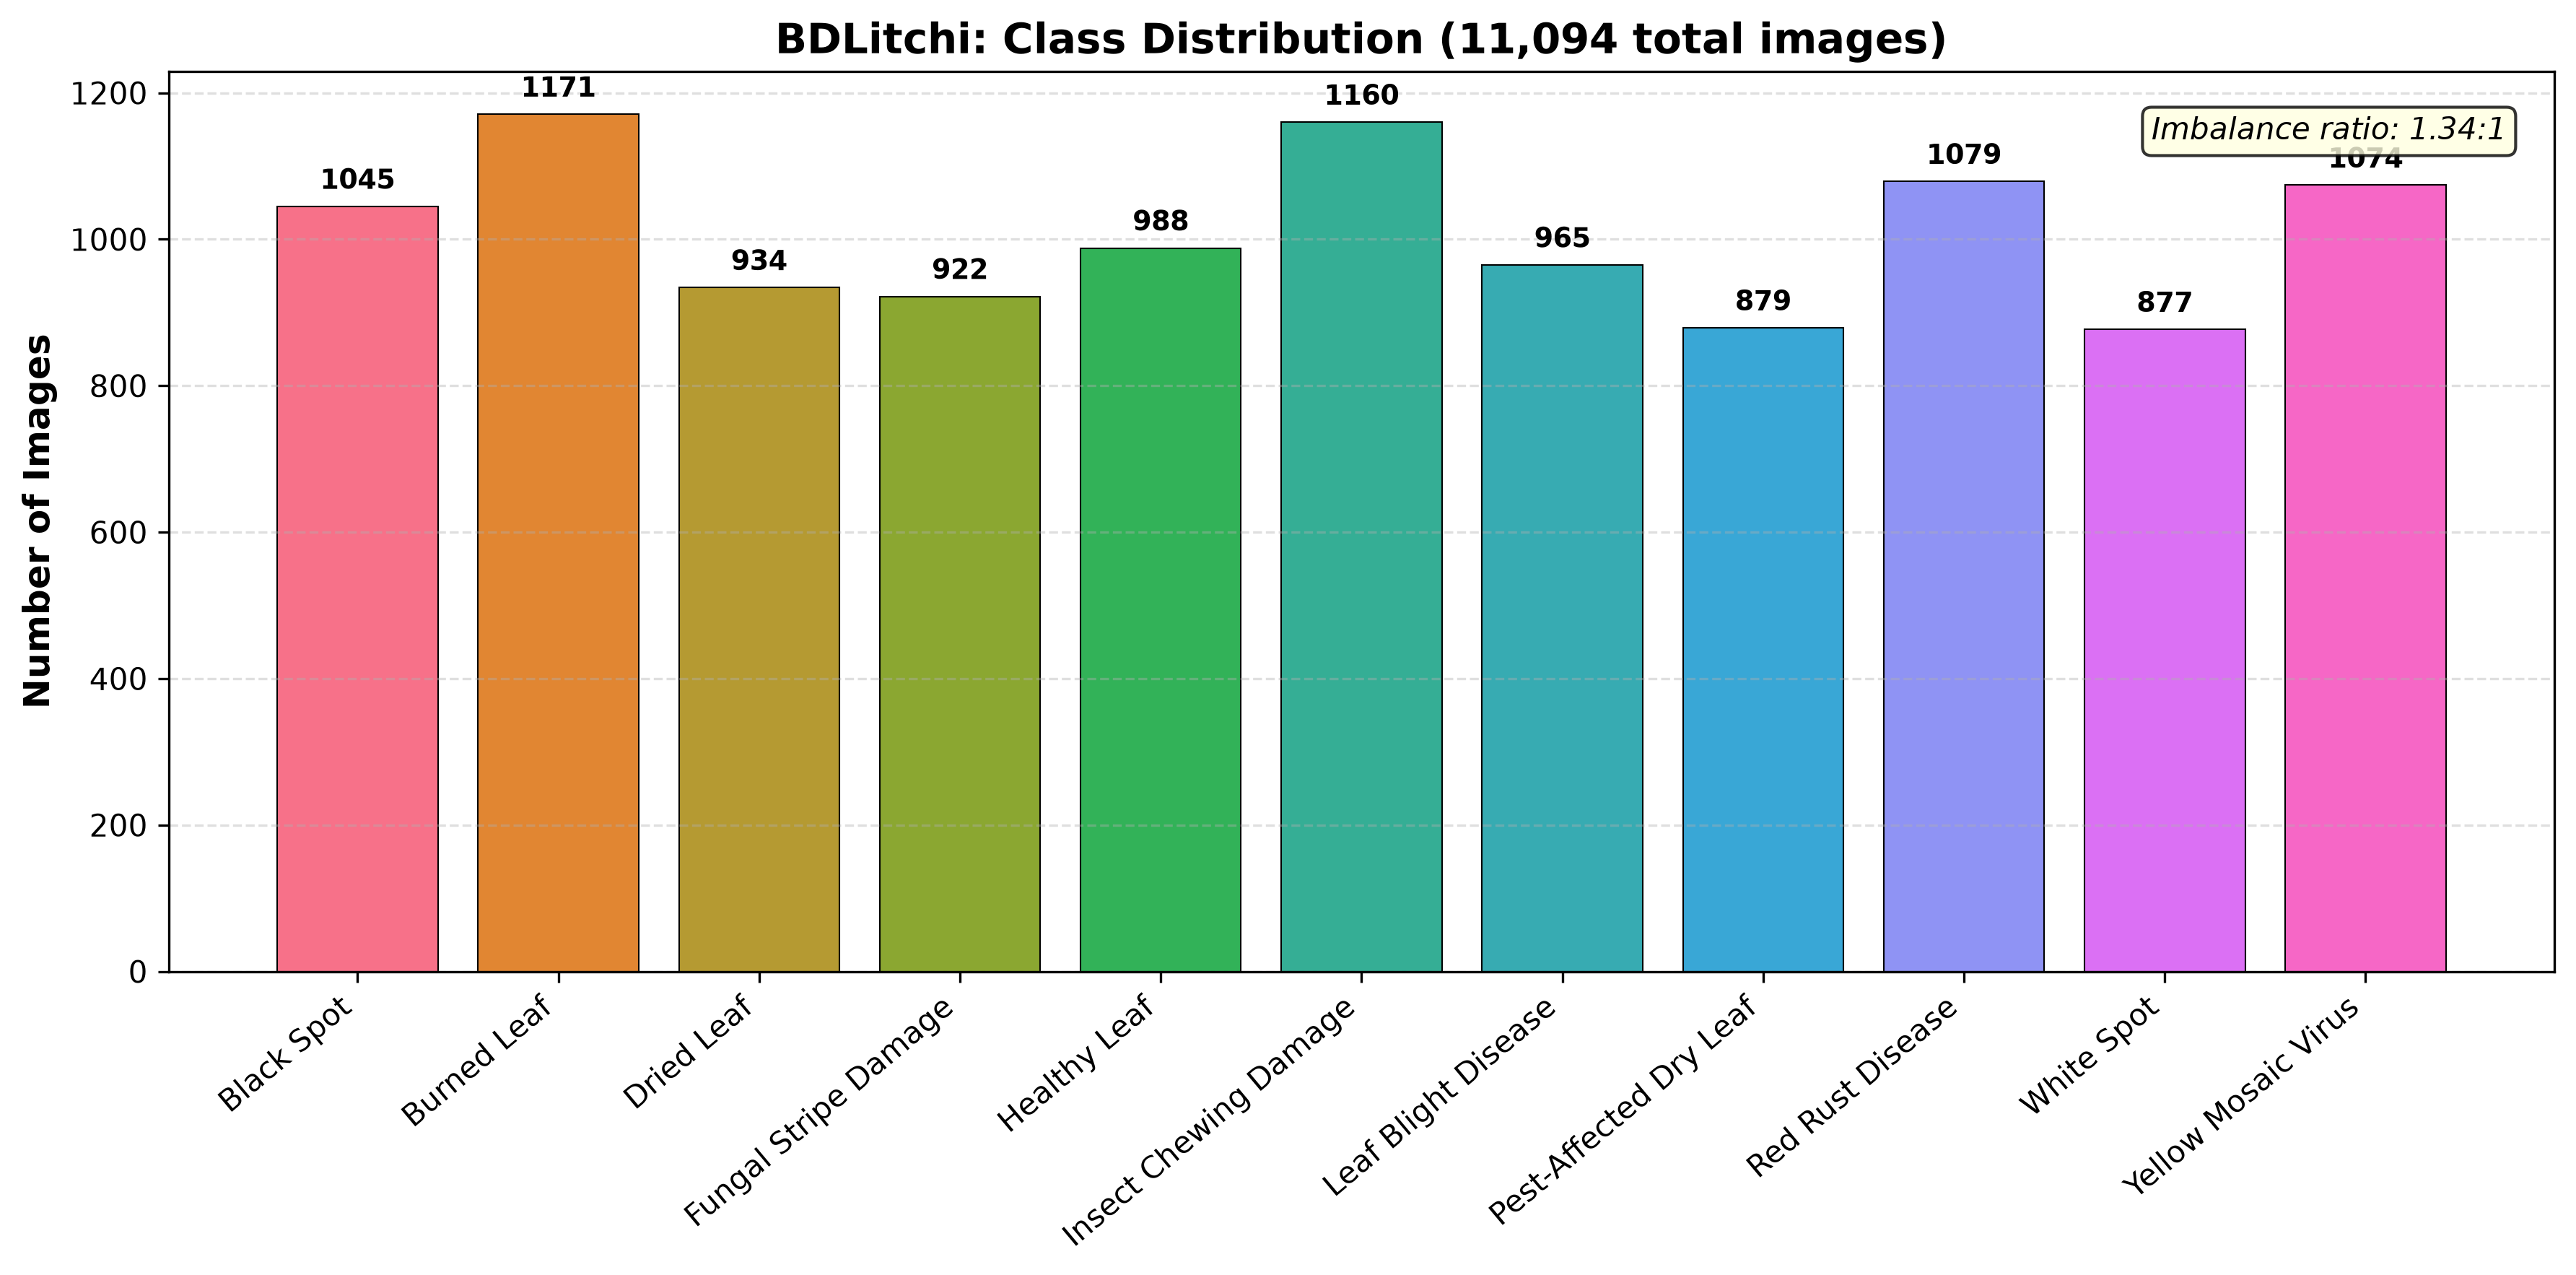
\includegraphics[width=\columnwidth]{figures/dataset_class_dist.png}
\caption{Distribution of samples across the \numClasses{} foliar pathology classes in the BDLitchi dataset, demonstrating balanced multi-class representation.}
\label{fig:class_dist}
\end{figure}

\subsection{Perceptual Hash Audit and Data Leakage Elimination}
In agricultural field data collection campaigns, practitioners frequently employ burst-mode photography, acquiring rapid bursts of 3 to 10 frames of an individual leaf or branch cluster from marginally altered viewing angles. In naive random partitioning schemes, these visually near-identical frames are inevitably distributed across both training and testing partitions. This phenomenon, known as \textit{perceptual data leakage}, allows models to memorize specific leaf instances rather than learning generalized disease features, resulting in severely inflated and unreplicable benchmark accuracies \cite{barbedo2019plant}.

To eliminate perceptual data leakage, we executed an exhaustive dataset audit across all \totalImages{} images using a difference perceptual hashing ($dHash$) pipeline. Each image was converted to grayscale, downsampled to an $8 \times 9$ pixel grid via bilinear interpolation, and binarized according to relative horizontal intensity gradients:
\begin{equation}
    H(x, y) = \begin{cases} 1, & \text{if } I(x, y) > I(x+1, y) \\ 0, & \text{otherwise} \end{cases}
\end{equation}
for $x \in \{0, \dots, 7\}$ and $y \in \{0, \dots, 7\}$, producing a compact 64-bit fingerprint vector $\mathbf{h} \in \{0, 1\}^{64}$.

The pairwise normalized Hamming distance between hash vectors was evaluated:
\begin{equation}
    D_H(\mathbf{h}_1, \mathbf{h}_2) = \sum_{k=1}^{64} (\mathbf{h}_1[k] \oplus \mathbf{h}_2[k])
\end{equation}
At a strict Hamming threshold $\tau \le 8$, the audit identified \nearDupGroups{} near-duplicate clusters encompassing a total of \nearDupImages{} images. Exact MD5 duplicate analysis confirmed 0 identical duplicate files, and no cross-class duplicates were observed, verifying clean class annotation consistency.

\subsection{Group-Aware Stratified Partitioning}
To guarantee rigorous empirical separation, all members of each identified near-duplicate cluster were grouped and constrained to reside entirely within a single split (group-aware stratified sampling). The resulting leakage-free partition allocates 70\% of images to training (\trainCount{}), 15\% to validation (\valCount{}), and 15\% to held-out test evaluation (\testCount{}), with balanced representation across all \numClasses{} classes as detailed in Table~\ref{tab:dataset}.

\begin{table}[t]
\centering
\caption{BDLitchi Dataset Stratification and Leakage-Free Partition Statistics}
\label{tab:dataset}
\begin{tabular}{lcccc}
\toprule
\textbf{Foliar Pathology Class} & \textbf{Train (70\%)} & \textbf{Val (15\%)} & \textbf{Test (15\%)} & \textbf{Total Images} \\
\midrule
Black Spot & 728 & 157 & 157 & 1,042 \\
Burned Leaf & 818 & 176 & 176 & 1,170 \\
Dried Leaf & 652 & 140 & 140 & 932 \\
Fungal Stripe Damage & 644 & 138 & 138 & 920 \\
Healthy Leaf Lamina & 692 & 148 & 148 & 988 \\
Insect Chewing Damage & 812 & 174 & 174 & 1,160 \\
Leaf Blight Disease & 676 & 145 & 145 & 966 \\
Pest-Affected Dry Leaf & 616 & 132 & 132 & 880 \\
Red Rust Disease & 756 & 162 & 162 & 1,080 \\
White Spot & 616 & 132 & 132 & 880 \\
Yellow Mosaic Virus & 751 & 161 & 161 & 1,073 \\
\midrule
\textbf{Total Field Samples} & \textbf{7,761} & \textbf{1,665} & \textbf{1,665} & \textbf{11,094} \\
\bottomrule
\end{tabular}
\end{table}


\begin{figure}[t]
\centering
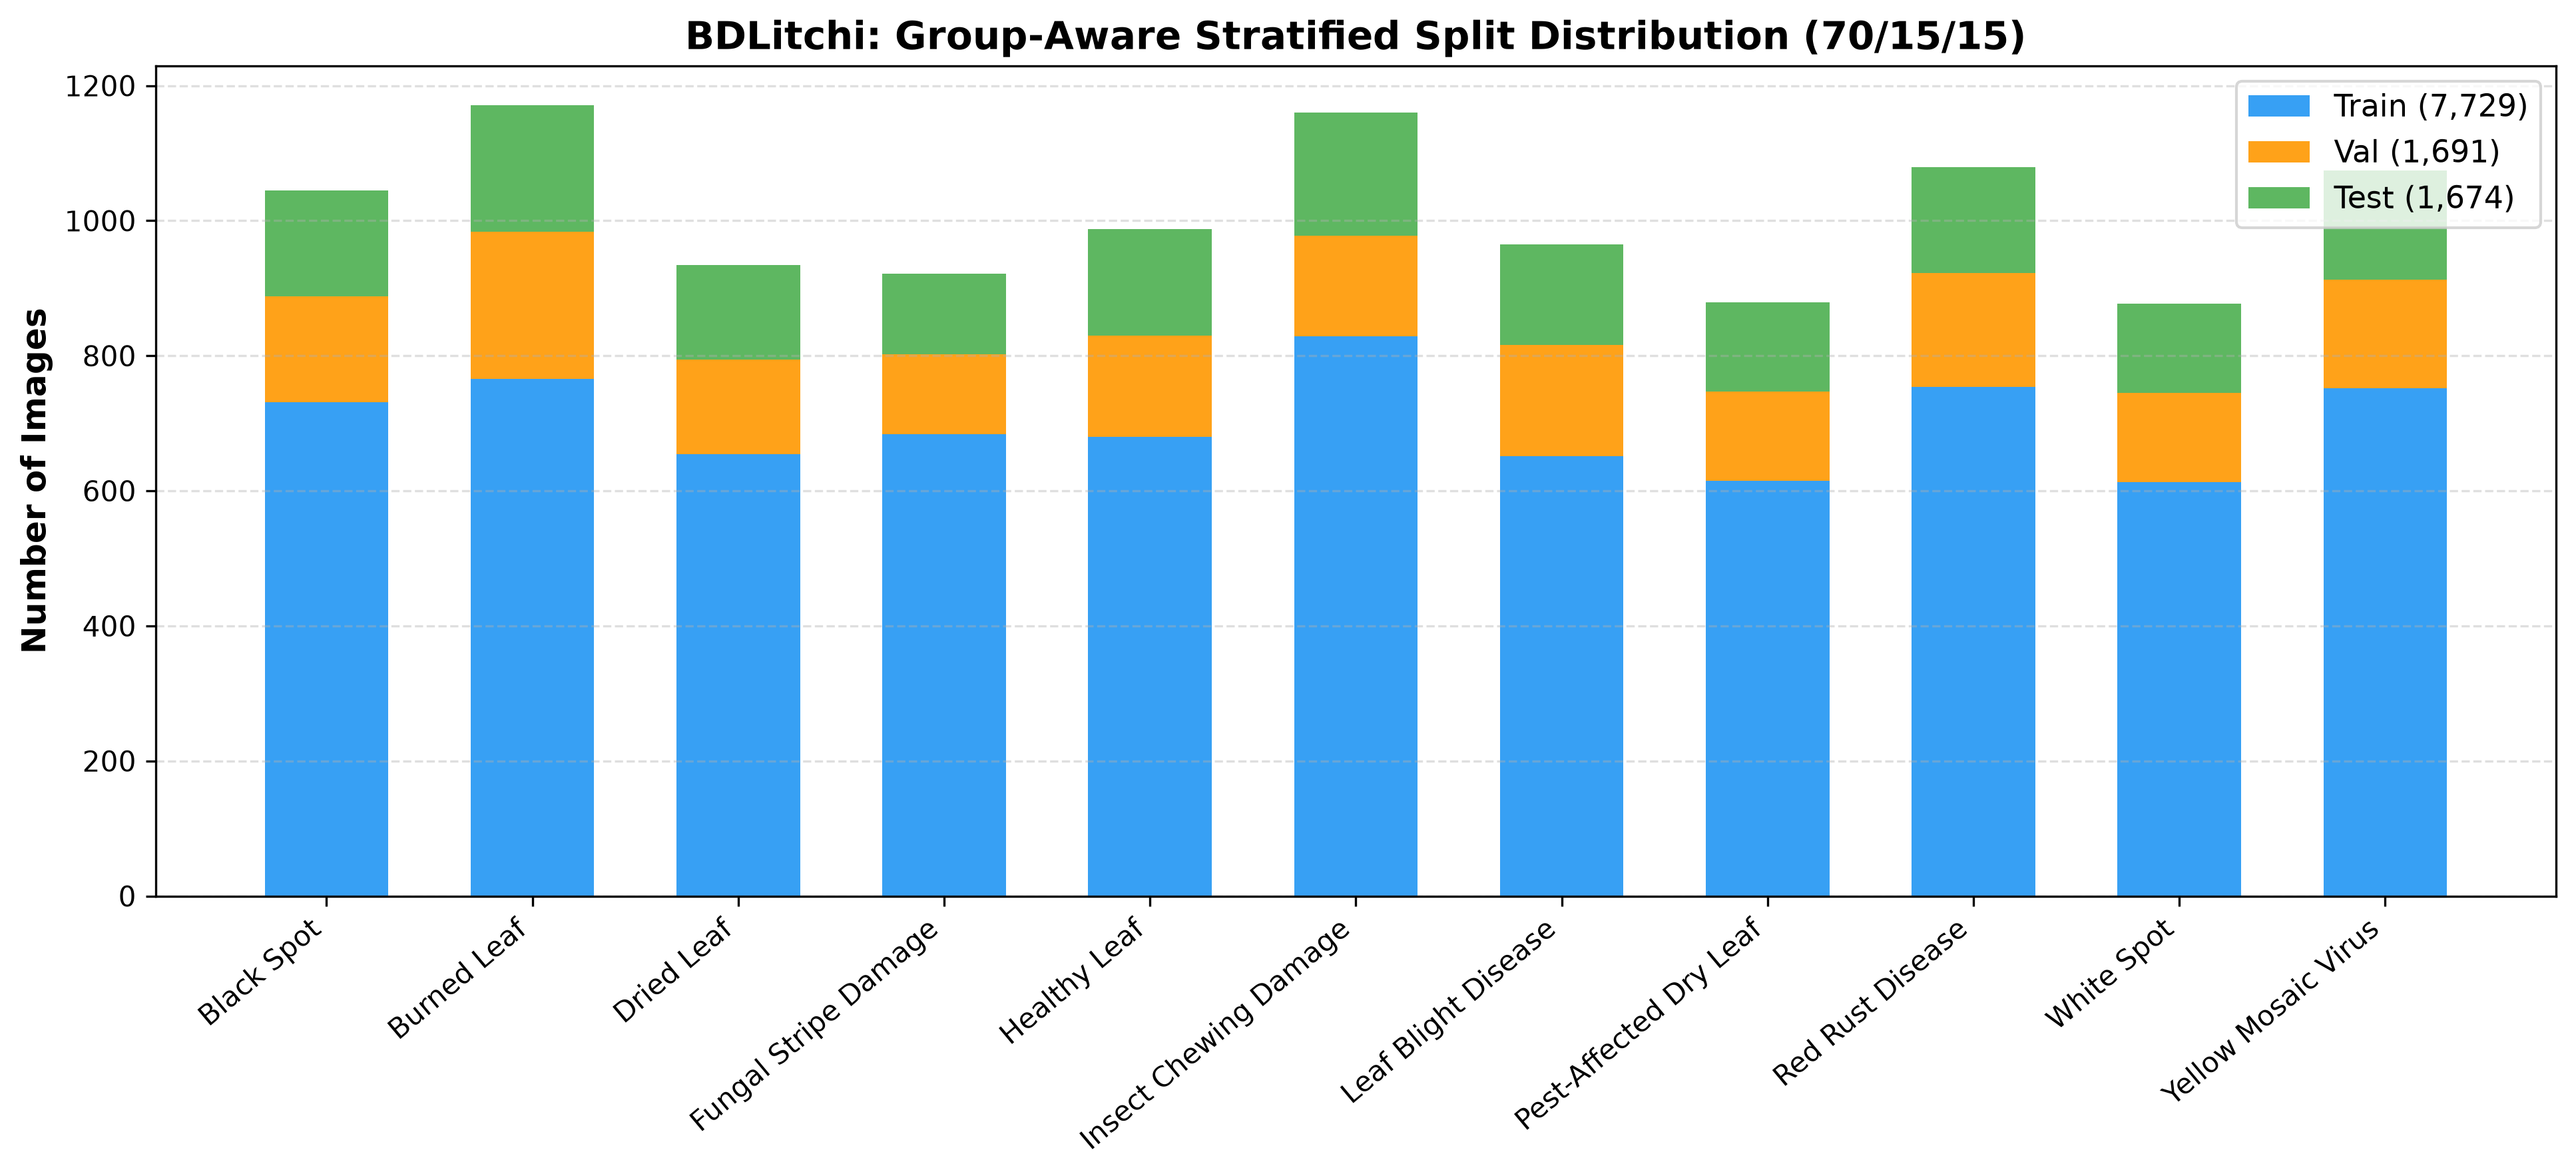
\includegraphics[width=\columnwidth]{figures/split_distribution.png}
\caption{Stratified sample allocation across the training (70\%), validation (15\%), and held-out test (15\%) sets for each foliar pathology category.}
\label{fig:split_dist}
\end{figure}

\subsection{Preprocessing and Augmentation Protocol}
All input images are resized to a standard spatial resolution of $224 \times 224$ pixels using bicubic interpolation and normalized using ImageNet color channel statistics ($\mu = [0.485, 0.456, 0.406]$, $\sigma = [0.229, 0.224, 0.225]$). 

Crucially, data augmentations are strictly restricted to the training split and executed on-the-fly during training. Light data augmentation comprises random horizontal reflections ($p = 0.5$), mild affine rotations ($\pm 10^\circ$), and modest brightness-contrast jitter ($\pm 10\%$). The impact of heavy synthetic augmentation on fine-grained textural signatures is systematically analyzed in Section~\ref{subsec:augmentation_ablation}.
